\documentclass[openany,a4paper,10pt]{book}

% Define the version number here
% This is automatically incremented when using the commitAll.sh script.
\newcommand{\version}{Version 0.001}

\usepackage[utf8]{inputenc}
\usepackage{amsmath,amssymb, amscd,amsbsy, amsthm, enumerate}
\usepackage{graphicx}
\usepackage{geometry}
\usepackage{titlesec}
\usepackage{lipsum}
\usepackage{wrapfig}
\usepackage{multicol}
\usepackage{listings}
\usepackage{xcolor}
\usepackage{appendix}

%used for custom page headers and page numbering
\usepackage{fancyhdr}

\usepackage{hyperref}

%enables indexing
\usepackage{makeidx}


\usepackage[T1]{fontenc}

\usepackage{tabularx}
%\renewcommand{\chaptername}{}

%\titleformat{\chapter}[display]{\normalfont\bfseries}{}{0pt}{\huge}

\geometry{margin=1in}

\setlength{\parindent}{25pt}

\renewcommand\bibname{References}

\renewcommand{\headrulewidth}{0pt}
%\setcounter{chapter}{-1} %starts the chapter labels at 0 instead of 1

\definecolor{backcolour}{rgb}{0.95,0.95,0.92}
\definecolor{commentcolour}{rgb}{.00,.245,.0}
\definecolor{lightgray}{gray}{0.9}
\lstdefinestyle{sharpc}{language=[Sharp]C, tabsize=3, backgroundcolor=\color{backcolour},breaklines=true, basicstyle=\footnotesize, showstringspaces=false, commentstyle=\color{commentcolour}, keywordstyle=\color{blue}}
\lstset{style=sharpc}


%%% This defines the note environment for you to write your solutions.
\newenvironment{note}
{\let\oldqedsymbol=\qedsymbol
	\renewcommand{\qedsymbol}{$ $}
	\begin{proof}[\bfseries\upshape \color{red}Note]\color{red}}
	{\end{proof}
	\renewcommand{\qedsymbol}{\oldqedsymbol}}

\newcommand{\inlinecode}[1]{\colorbox{lightgray}{\lstinline{#1}}}




%%Different lstlisting formats go here

% Define the custom terminal style
\lstdefinestyle{terminalstyle}{
	language=bash,                   % Set the language to Bash
	basicstyle=\ttfamily\color{white}, % Use a monospaced font and white text
	backgroundcolor=\color{black},   % Background color
	frame=tb,                        % Top and bottom frame lines
	framerule=0.5pt,                 % Frame rule width
	xleftmargin=5pt,                % Left margin
	xrightmargin=0pt,                % Right margin
	rulecolor=\color{black!20},      % Frame color
	showstringspaces=false,          % Don't show spaces in strings
	upquote=true,                    % Use straight quotes
	commentstyle=\color{green},      % Comments are green
	keywordstyle=\color{orange!60},  % Keywords
	numbers=left,                    % Line numbers on the left
	numberstyle=\tiny\color{black!90},   % Line number style
	captionpos=b,                    % Caption position (bottom)
	breaklines=true,                 % Automatically break long lines
	postbreak=\mbox{\textcolor{green}{$\hookrightarrow$}\space}, % Line continuation symbol
}

% Define a bash/shell style.
\lstdefinestyle{shellstyle}{
	language=sh,                    % Set the language to Shell
	basicstyle=\ttfamily,           % Use a monospaced font
	backgroundcolor=\color{gray!10},% Background color
	keywordstyle=\color{blue},      % Keywords are blue
	commentstyle=\color{green!40!black}, % Comments are green
	stringstyle=\color{red},        % Strings are red
	rulecolor=\color{black},        % Frame color
	breakatwhitespace=false,        % Don't break lines at whitespace
	breaklines=true,                % Automatically break long lines
	postbreak=\mbox{\textcolor{red}{$\hookrightarrow$}\space}, % Line continuation symbol
	showstringspaces=false,         % Don't show spaces in strings
	captionpos=b,                   % Caption position (bottom)
	frame=single,                   % Add a frame around listings
	numbers=left,                   % Line numbers on the left
	numberstyle=\tiny\color{gray},  % Line number style
	stepnumber=1,                   % Line number increments
	tabsize=4,                      % Tab size
	xleftmargin=5pt,               % Left margin
	xrightmargin=0pt                % Right margin
}

% Define Python style
\lstdefinestyle{pythonstyle}{
	language=Python,
	basicstyle=\ttfamily\small,
	numbers=left,
	numberstyle=\tiny\color{gray},
	frame=single,
	rulecolor=\color{orange},
	backgroundcolor=\color{orange!05},
	keywordstyle=\color{blue},
	commentstyle=\color{green!40!black},
	stringstyle=\color{red},
	breaklines=true,
	tabsize=4,
	captionpos=b,
	extendedchars=true,
	inputencoding=utf8,
	showspaces=false,
	showstringspaces=false,
	xleftmargin=5pt,               % Left margin
	xrightmargin=0pt                % Right margin
}


% Define C++ style
\lstdefinestyle{cppstyle}{
	language=C++,
	basicstyle=\ttfamily\small,
	numbers=left,
	numberstyle=\tiny\color{gray},
	frame=single,
	rulecolor=\color{black!30},
	backgroundcolor=\color{gray!05},% Background color
	keywordstyle=\color{blue},
	commentstyle=\color{green!40!black},
	stringstyle=\color{red},
	breaklines=true,
	tabsize=4,
	captionpos=b,
	extendedchars=true,
	inputencoding=utf8,
	showspaces=false,
	showstringspaces=false,
	xleftmargin=5pt,               % Left margin
	xrightmargin=0pt                % Right margin
}

% Define dark green color
\definecolor{darkgreen}{RGB}{0,100,0}

% Define Makefile style
\lstdefinestyle{makestyle}{
	language=make,
	basicstyle=\ttfamily\small,
	numbers=left,
	numberstyle=\tiny\color{gray},
	frame=single,
	backgroundcolor=\color{darkgreen!05},
	rulecolor=\color{darkgreen},
	keywordstyle=\color{blue},
	commentstyle=\color{green!40!black},
	stringstyle=\color{red},
	breaklines=true,
	tabsize=4,
	captionpos=b,
	extendedchars=true,
	inputencoding=utf8,
	showspaces=false,
	showstringspaces=false,
	xleftmargin=5pt,               % Left margin
	xrightmargin=0pt                % Right margin
}

% Define Git style
\lstdefinestyle{gitstyle}{
	language=bash, % Assuming Git commands are written in a bash-like language
	basicstyle=\ttfamily\small,
	numbers=left,
	numberstyle=\tiny\color{gray},
	frame=single,
	backgroundcolor=\color{blue!05},
	rulecolor=\color{blue},
	keywordstyle=\color{blue},
	commentstyle=\color{green!40!black},
	stringstyle=\color{red},
	breaklines=true,
	tabsize=4,
	captionpos=b,
	extendedchars=true,
	inputencoding=utf8,
	showspaces=false,
	showstringspaces=false,
	xleftmargin=5pt,               % Left margin
	xrightmargin=0pt                % Right margin
}

% Define C# style
\lstdefinestyle{csharpstyle}{
	language=[Sharp]C,
	basicstyle=\ttfamily\small,
	numbers=left,
	numberstyle=\tiny\color{gray},
	frame=single,
	rulecolor=\color{purple},
	backgroundcolor=\color{purple!05},
	keywordstyle=\color{blue},
	commentstyle=\color{green!40!black},
	stringstyle=\color{red},
	breaklines=true,
	tabsize=4,
	captionpos=b,
	extendedchars=true,
	inputencoding=utf8,
	showspaces=false,
	showstringspaces=false,
	xleftmargin=5pt,               % Left margin
	xrightmargin=0pt                % Right margin
}

% Define Java style
\lstdefinestyle{javastyle}{
	language=Java,
	basicstyle=\ttfamily,
	keywordstyle=\color{blue},
	rulecolor=\color{red!80},
	backgroundcolor=\color{red!05},
	commentstyle=\color{green!70!black},
	stringstyle=\color{red},
	numbers=left,
	numberstyle=\tiny\color{gray},
	stepnumber=1,
	breaklines=true,
	breakatwhitespace=false,
	tabsize=4,
	frame=single,
	showspaces=false,
	showstringspaces=false,
	xleftmargin=5pt,               % Left margin
	xrightmargin=0pt                % Right margin
}

% Define JavaScript language settings
\lstdefinelanguage{JavaScript}{
	keywords={typeof, new, true, false, catch, function, return, null, catch, switch, var, if, in, while, do, else, case, break, default},
	keywordstyle=\color{blue}\bfseries,
	ndkeywords={class, export, boolean, throw, implements, import, this},
	ndkeywordstyle=\color{darkgray}\bfseries,
	identifierstyle=\color{black},
	sensitive=false,
	comment=[l]{//},
	morecomment=[s]{/*}{*/},
	commentstyle=\color{purple}\ttfamily,
	stringstyle=\color{red}\ttfamily,
	morestring=[b]',
	morestring=[b]",
}

% Define JavaScript style
\lstdefinestyle{jsstyle}{
	language=JavaScript,
	basicstyle=\ttfamily,
	rulecolor=\color{red!80},
	backgroundcolor=\color{red!05},
	keywordstyle=\color{blue},
	commentstyle=\color{green!70!black},
	stringstyle=\color{red},
	numbers=left,
	numberstyle=\tiny\color{gray},
	stepnumber=1,
	breaklines=true,
	breakatwhitespace=false,
	tabsize=4,
	frame=single,
	showspaces=false,
	showstringspaces=false,
	xleftmargin=5pt,               % Left margin
	xrightmargin=0pt                % Right margin
}

% Define HTML style
\lstdefinestyle{htmlstyle}{
	language=HTML,
	basicstyle=\ttfamily\small,
	numbers=left,
	numberstyle=\tiny\color{gray},
	frame=single,
	rulecolor=\color{black},
	backgroundcolor=\color{yellow!05},
	keywordstyle=\color{blue},
	commentstyle=\color{green!40!black},
	stringstyle=\color{red},
	breaklines=true,
	tabsize=4,
	captionpos=b,
	extendedchars=true,
	inputencoding=utf8,
	showspaces=false,
	showstringspaces=false,
	xleftmargin=5pt,               % Left margin
	xrightmargin=0pt                % Right margin
}

% Define CSS style
\lstdefinestyle{cssstyle}{
	language=HTML,
	basicstyle=\ttfamily\small,
	numbers=left,
	numberstyle=\tiny\color{gray},
	frame=single,
	rulecolor=\color{black},
	keywordstyle=\color{blue},
	commentstyle=\color{green!40!black},
	stringstyle=\color{red},
	breaklines=true,
	tabsize=4,
	captionpos=b,
	extendedchars=true,
	inputencoding=utf8,
	showspaces=false,
	showstringspaces=false,
	xleftmargin=5pt,               % Left margin
	xrightmargin=0pt                % Right margin
}

% Define LaTeX style
\lstdefinestyle{latexstyle}{
	language=TeX,
	basicstyle=\ttfamily\small,
	numbers=left,
	numberstyle=\tiny\color{gray},
	frame=single,
	rulecolor=\color{brown},
	backgroundcolor=\color{brown!05},
	keywordstyle=\color{blue},
	commentstyle=\color{green!40!black},
	stringstyle=\color{red},
	breaklines=true,
	tabsize=4,
	captionpos=b,
	extendedchars=true,
	inputencoding=utf8,
	showspaces=false,
	showstringspaces=false,
	xleftmargin=5pt,               % Left margin
	xrightmargin=0pt                % Right margin
}

% Define PHP style
\lstdefinestyle{phpstyle}{
	language=PHP,
	basicstyle=\ttfamily\small,
	numbers=left,
	numberstyle=\tiny\color{gray},
	frame=single,
	rulecolor=\color{black},
	keywordstyle=\color{blue},
	commentstyle=\color{green!40!black},
	stringstyle=\color{red},
	breaklines=true,
	tabsize=4,
	captionpos=b,
	extendedchars=true,
	inputencoding=utf8,
	showspaces=false,
	showstringspaces=false,
	xleftmargin=5pt,               % Left margin
	xrightmargin=0pt                % Right margin
}

\title{\vspace{0.1cm}  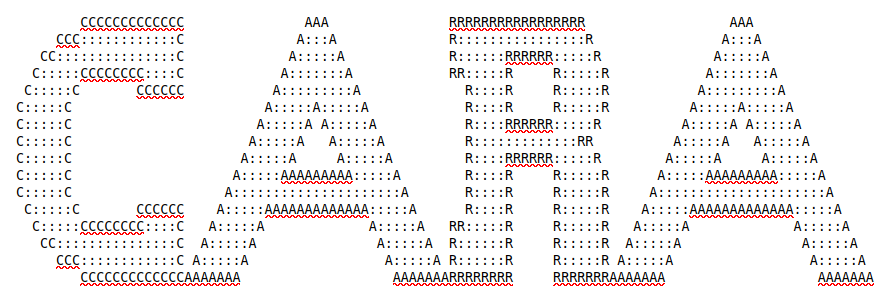
\includegraphics[scale=0.6]{./images/cara_cover.png} \vspace{.5cm} \\ Changelog Automation \& Release Assistant (CARA) \\  Manual \& Programming Documentation}
\author{Developer: Antonius Torode}
\date{Version -- \version \\ Latest update: \today}

\makeindex

\begin{document}

\frontmatter
\maketitle
\pagestyle{empty}
%% copyrightpage
\begingroup
\footnotesize
\parindent 0pt
\parskip \baselineskip
\textcopyright{} 2025 Antonius Torode \\
All rights reserved.

This work may be distributed and/or modified under the conditions of Antonius’ General Purpose License (AGPL).

The Original Maintainer of this work is: Antonius Torode.

The Current Maintainer of this work is: Antonius Torode.

This document is intended solely to provide documentation for the Changelog Automation \& Release Assistant (CARA), a tool developed to automate changelog generation and formatting using Git history. Throughout this document, "CARA" will refer to the Changelog Automation \& Release Assistant. This tool was created for configurable changelog output and supports multiple logging and formatting schemes for software projects. This project is hosted at the following URL:

\begin{center}
	\url{https://github.com/torodean/CARA}
\end{center}


\begin{center}
\begin{tabular}{ll}
This document is continuously under development. \\
Most Current Revision Date: &  \today 
\end{tabular}
\end{center}

\vfill

Torode, A.\\
\hspace*{1em} CARA Documentation. \\
\hspace*{2em} 2025. \\
\hspace*{2em} Includes Source Code and References \\


\endgroup
\clearpage
\tableofcontents
\newpage
\vspace*{\fill}
\begin{center}
	\textit{This page intentionally left blank. \\(Yes, this is a contradiction)}
\end{center}
\vspace*{\fill}

\mainmatter
\pagestyle{fancy}
\fancyhf{}
\fancyhead[RO, LE]{\thepage}


\fancypagestyle{plain}{%
	%\fancyhf{} % clear all header and footer fields
	\fancyhead[RO, LE]{\thepage}
	\renewcommand{\headrulewidth}{0pt}
	\renewcommand{\footrulewidth}{0pt}}

\chapter{Introduction}
\label{ch:introduction}
\pagestyle{fancy}

The \textbf{Changelog Automation \& Release Assistant (CARA)} is a command-line tool designed to automate the process of generating and maintaining changelogs using Git commit history. CARA parses Git logs and formats the output according to a customizable configuration, allowing users to streamline their release documentation process.

CARA supports multiple verbosity levels, debug output, and configurable input/output paths, making it adaptable to a variety of development workflows. It is intended for developers who maintain changelogs regularly and prefer consistency, automation, and clarity in their version history tracking.


















\section{How to Use CARA}

To use \textbf{CARA}, ensure the main script \texttt{cara.py} and a configuration file (e.g., \texttt{cara.conf}) are present in your project directory. The configuration file specifies options such as grouping method, output format, filtering rules, and more. See chapter \ref{ch:configuration} for more details on the configuration file. Once configured, run the script from your project's root directory using:
\begin{lstlisting}[style=terminalstyle]
python3 /path/to/cara.py -c /path/to/cara.conf
\end{lstlisting}
CARA will parse your Git commit history, group entries according to your configuration (e.g., by day or week), filter out undesired commits, and generate a structured changelog. The output will be written to the file path specified in your command. For full details on configuration options, refer to the documentation in the \texttt{docs/} directory. Various other optional program arguments are available which can be accessed via the \texttt{-h} flag:
\begin{lstlisting}[style=terminalstyle]
$ python3 cara.py -h
usage: cara.py [-h] [-v] [-d] [-c CONFIG] [-i INPUT] [-o OUTPUT] [-r REPO]

Changelog Automation & Release Assistant (CARA).

optional arguments:
  -h, --help            show this help message and exit
  -v, --verbose         Enables verbose mode. This will output various program data for
                        detailed output.
  -d, --debug           Enables debug mode. This will output various program data for
                        debugging.
  -c CONFIG, --config CONFIG
                        The configuration file to use.
  -i INPUT, --input INPUT
                        The input changelog to use. Use this option to overwrite/update an
                        existing changelog.
  -o OUTPUT, --output OUTPUT
                        The output file to use. Use this option to create a new changelog.
  -r REPO, --repo REPO  The repo path to use. This will default to the current directory.
\end{lstlisting}
\chapter{Configuration}
\label{ch:configuration}
\pagestyle{fancy}

The CARA configuration system allows users to define how changelogs are generated and formatted. Configuration files provide a flexible and human-readable way to customize the behavior of the application without modifying the source code.

CARA reads configuration data from a plain text file, where each line defines a key-value pair separated by an equals sign (`=`). Lines beginning with `\#` are treated as comments and ignored. Empty lines and improperly formatted entries are also skipped during parsing.

The configuration system is implemented through the \texttt{Config} class, which is responsible for loading, parsing, and storing configuration values. Users can specify a configuration file at runtime via the \texttt{--config} flag. Once loaded, the configuration can be queried programmatically or used internally to guide CARA’s behavior. To use the default behavior for any configuration option, simply omit or comment out the option from the configuration file.

The expected format for configuration entries is:

\begin{lstlisting}[style=cppstyle]
key=value  # Optional comment.
\end{lstlisting}

This format provides clarity and simplicity, ensuring easy editing and version control. Each configuration key corresponds to a specific setting or feature within CARA, as documented in subsequent sections of this chapter.















\section{DATE\_FORMAT Configuration Option}

The \texttt{DATE\_FORMAT} option in the configuration file allows users to control the format in which commit dates are displayed in the generated changelog. This option directly maps to the \texttt{--date=format:<str>} flag in \texttt{git log}, enabling a wide range of formatting options based on user preferences or documentation standards. If this option is defined in the configuration file, CARA will invoke \texttt{git log} with the specified format string. Otherwise, Git's default date formatting is used.

\begin{lstlisting}[style=cppstyle]
// Example Configuration
DATE_FORMAT=%Y-%m-%d
\end{lstlisting}

\subsection*{Common Format Examples}
\begin{itemize}
	\item \texttt{\%Y-\%m-\%d} – 2025-07-01 (ISO standard)
	\item \texttt{\%d-\%m-\%Y} – 01-07-2025 (European)
	\item \texttt{\%B \%d, \%Y} – July 01, 2025 (Verbose)
	\item \texttt{\%a \%Y-\%m-\%d at \%H:\%M} – Tue 2025-07-01 at 14:30
\end{itemize}

For the full list of supported format tokens, refer to the \texttt{strftime(3)}\cite{strftime(3)} man page or Git's documentation on custom date formats.










\section{GROUP\_BY Configuration Option}
\label{sec:groupby}

The \texttt{GROUP\_BY} configuration value determines how commit entries in the generated changelog are grouped. Grouping provides structure to the changelog output by organizing commits into logical sections based on time.

\subsection*{Accepted Values}
\begin{itemize}
	\item \texttt{day} --- Groups commits by individual date (e.g., \texttt{2025-07-01}).
	\item \texttt{week} --- Groups commits by ISO calendar week (e.g., \texttt{2025-W27}).
	\item \texttt{month} --- Groups commits by calendar month (e.g., \texttt{2025-07}).
	\item \texttt{year} --- Groups commits by year (e.g., \texttt{2025}).
\end{itemize}

\subsection*{Default Behavior}
If this configuration value is not set, the default grouping is by \texttt{day}.

\subsection*{Usage}
This option affects the organization of the changelog. Each group is rendered as a section in the output, prefixed with a heading containing the grouping key (e.g., date or week label). Commits within each group are listed chronologically.









\section{OUTPUT\_ENTRIES Configuration Option}

The \texttt{OUTPUT\_ENTRIES} configuration option controls which fields are included for each commit entry in the generated changelog output. This value should be a space-separated list of field names, allowing flexible control over the formatting of each entry.

\subsection*{Valid Fields:}
\begin{itemize}
	\item \texttt{commit} -- Includes the full commit hash.
	\item \texttt{author} -- Includes the name of the author who made the commit.
	\item \texttt{message} -- Includes the commit message.
\end{itemize}

\subsection*{Special Value:}
\begin{itemize}
	\item \texttt{all} -- A shortcut that includes all of the above fields in the default format.
\end{itemize}

\subsection*{Example Values:}
\begin{itemize}
	\item \texttt{OUTPUT\_ENTRIES=commit message}
	\item \texttt{OUTPUT\_ENTRIES=author}
	\item \texttt{OUTPUT\_ENTRIES=all}
\end{itemize}

Each selected field will be printed in order, separated by colons and dashes according to default formatting. This allows for compact or verbose output depending on user preference.














\subsection{Filtering Configuration Options}

The changelog generator supports several filtering options to control which commit messages are included in the final output. These options allow users to exclude trivial or irrelevant commits and focus on meaningful changes.

\begin{description}
	\item[MIN\_WORDS] Specifies the minimum number of words required in a commit message for it to be included. If the message contains fewer words, it will be discarded. This option takes priority over \texttt{MIN\_CHARS} if both are set.
	
	\item[MIN\_CHARS] Specifies the minimum number of characters required in a commit message. If the message is shorter than this length, it will be excluded. Ignored if \texttt{MIN\_WORDS} is also set.
	
	\item[EXCLUDE\_KEYWORDS] A space-separated list of keywords. If any of these appear in a commit message (case-insensitive), the message will be excluded from the output.
	
	\item[INCLUDE\_KEYWORDS] A space-separated list of required keywords. Only commit messages containing at least one of these keywords (case-insensitive) will be included. If not set, this filter is ignored.
\end{description}

These options provide a flexible way to tailor the changelog content by filtering out uninformative or irrelevant commits.






\backmatter
%\begin{appendices}

\end{appendices}






%\begin{thebibliography}{99}
	\bibitem{item} 
\end{thebibliography}
\printindex


\end{document}
